\documentclass[12pt,a4paper]{article}
% \usepackage[utf8]{inputenc} % fontspecと併用時は不要
\usepackage[japanese]{babel}
\usepackage{amsmath}
\usepackage{amsfonts}
\usepackage{amssymb}
\usepackage{empheq}
\usepackage{geometry}
\usepackage{graphicx}
\usepackage{enumitem}
\usepackage{fancyhdr}
\usepackage{verbatim}
\usepackage{tcolorbox}
\tcbuselibrary{breakable}

% 日本語改行設定
\usepackage{xeCJK}
\usepackage{indentfirst}
\setlength{\parindent}{1em}

% 日本語フォント設定
\usepackage{fontspec}
\setmainfont{Hiragino Mincho Pro}
\setsansfont{Hiragino Sans}
\setmonofont{Menlo}
\setCJKmainfont{Hiragino Mincho Pro}
\setCJKsansfont{Hiragino Sans}
\setCJKmonofont{Menlo}
% ページ設定
\geometry{margin=1.5cm}
\pagestyle{fancy}
\fancyhf{}
\fancyhead[L]{プログラミング応用 期末課題}
\fancyhead[R]{期末課題解説}
%\fancyfoot[R]{\ifnum\value{page}=1\small（裏面に続く）\fi}
\fancyfoot[C]{\thepage}
\renewcommand{\headrulewidth}{0.4pt}
\renewcommand{\footrulewidth}{0.4pt}

% 問題番号のカウンター
\newcounter{problem}
\setcounter{problem}{0}

% シンプルな問題環境
\newenvironment{problem}[1][]{
    \refstepcounter{problem}
    \vspace{1em}
    \noindent
    \textbf{問\arabic{problem}} #1
    %\vspace{0.5em}
    %\par
}{
    \vspace{1em}
}

% 解答環境
\newenvironment{solution}{
    \vspace{0.5em}
    \begin{tcolorbox}[colback=white, colframe=black, boxrule=1pt, arc=0mm, breakable]
    \noindent
    \textbf{【解答】}
    \vspace{0.3em}
}{
    \end{tcolorbox}
    \vspace{1em}
}

\begin{document}

% ヘッダー情報
\begin{center}
    {\Large \textbf{プログラミング応用}}\\[0.5em]
    {\large \textbf{期末課題 解説}}\\[1em]
\end{center}

\begin{problem}
グラフ $G=(V,E)$ がグラフ $H=(W,F)$ を含むとは, ある単射 $\phi\colon W\to V$ が存在して, 全ての$H$の辺 $\{a,b\}\in F$ に対して $\{\phi(a),\phi(b)\}\in E$ を満たすことを言う. 隣接行列として与えられた$n$頂点グラフ$G$が次の図\ref{fig:H}で表されるグラフ$H$を含むかどうかを判定する問題を考える.

  \begin{figure}[h]
    \begin{center}
    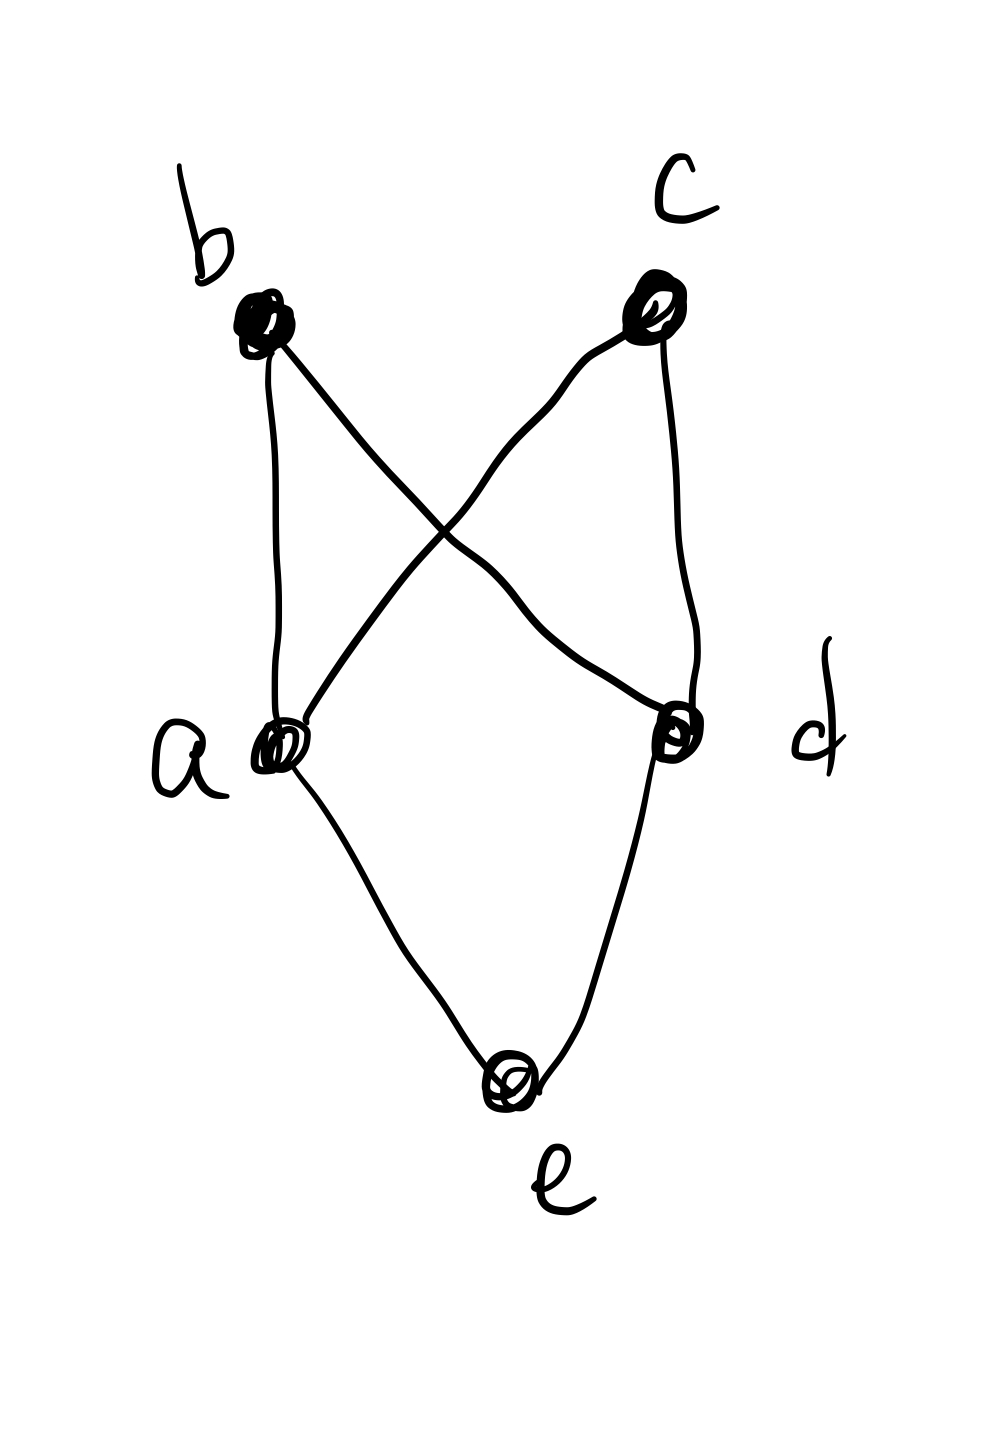
\includegraphics[width=0.14\textwidth]{H.png}
    \caption{グラフ $H$ \label{fig:H}}
    \end{center}
  \end{figure}

  \begin{enumerate}
    \item この問題を $O(n^3)$時間で判定するアルゴリズムを記述せよ. (\textbf{4点})
    \item この問題を $O(n^2)$時間で判定するアルゴリズムを記述せよ. (\textbf{6点})
  \end{enumerate}

\end{problem}

\begin{solution}
  \paragraph*{1の解説.}
  隣接行列$A$に対し, $A^2$を$O(n^3)$時間で計算し, $A^2_{u,v}\ge 3$を満たす$u\ne v$が存在するかどうかを確認すればよい.

    \paragraph*{2の解説.}  
  与えられたグラフを$G=(V,E)$とする. 頂点$u$の隣接頂点の集合を$N(u)$とする. 以下のアルゴリズムを考える:

\begin{enumerate}
  \item 二次元$n\times n$リスト $C$を用意し, 全ての成分を$0$で初期化する.
  \item 全ての$u\in V$に対して以下を実行する:
  \begin{enumerate}
    \item 全ての$v\in N(u)$に対して, $C_{u,v}\leftarrow C_{u,v}+1$とする.
    \item $C_{u,v}\ge 3$ならば, 「Yes」を出力して終了.
  \end{enumerate}
  \item 最後まで終了しなければ, 「No」を出力して終了.
  
\end{enumerate}

このアルゴリズムは$O(n^2)$時間で動作する. 実際, もしも2の反復が$2n^2+1$回実行されてもなお終了していないとき, $C$の成分の個数は$n^2$個なので, 必ずどこかの成分は$3$回以上$+1$されているはずであるが, その瞬間にアルゴリズムは終了するため, 矛盾する.

\end{solution}

\begin{problem}
$n$個の$n$次元ベクトル $A_1,\dots,A_n \in \mathbb{Z}^{n}$ が与えられる.ただし$n\ge 68$であり, ベクトル$A_i$の各成分の絶対値は高々$n^{100}$である. これらの中から相異なる$68$個のベクトルを選んでその総和を零ベクトルにできるかどうかを $O(n^{34}\log n)$時間で判定するアルゴリズムを記述せよ. (\textbf{10点})
\end{problem}

\begin{solution}
  与えられた入力を$A_1,\dots,A_n\in\mathbb{Z}^n$とする. 以下の乱択アルゴリズムを考える:
  \begin{enumerate}
    \item ベクトル$r\in\mathbb{Z}^n$を, 各成分を独立に$\{1, 2,\dots,100\cdot n^{68}\}$の中から一様ランダムに選んで得られるランダムベクトルとする.
    \item 各$i=1,\dots,n$に対し, $a_i := A_i^\top r$を計算する.
    \item 集合 $S=\{a_1,\dots,a_n\}$ (多重集合とみなす) をランダムに68個の部分集合に分割し, $S=S_1\sqcup \dots \sqcup S_{68}$とする.
    \item 各$S_i$から一つずつ$s_i\in S_i$を選び, $s_1+\dots+s_{68}=0$となるような$s_1,\dots,s_{68}$が存在するかどうかを$O(n^{34}\log n)$時間で判定し, もし存在するならばYesを出力して終了する. これは, 全ての$s_1\in S_1,\dots,s_{34}\in S_{34}$に対し, $s_1+\dots+s_{34}$を格納したリスト$L$を作り, これをソートした上で, 各$s_{35}\in S_{35},\dots,s_{68}\in S_{68}$に対し, $-(s_{35}+\dots+s_{68})$が$L$の属するかどうかを二分探索して存在するかどうかを確認すれば$O(n^{34}\log n)$時間で判定できる.
    \item ステップ3と4を十分大きな定数回, 具体的には $100\cdot \frac{68^{68}}{68!}$ 回だけ繰り返し, 一度もYesが出力されなければNoを出力して終了する.
  \end{enumerate}

  この乱択アルゴリズムは確かに$O(n^{34}\log n)$時間で動作する. また, この乱択アルゴリズムは以下を満たす:
  \begin{itemize}
    \item 入力$A_1,\dots,A_n$の答えがYesならば, この乱択アルゴリズムは確率$0.99$でYesを出力する.
    \item 入力$A_1,\dots,A_n$の答えがNoならば, この乱択アルゴリズムは確率$0.99$でNoを出力する.
  \end{itemize}
  これら二つの主張を証明すれば, 上記の乱択アルゴリズムが正しく問題を解くことが示されたことになる.
  
  一つ目の主張を証明する. 例えば$A_1+\dots+A_{68}=0$となるならば, ステップ2で得られる$a_1,\dots,a_{68}$は, $a_1+\dots+a_{68}=0$となる. さらに, これら68個のベクトルは, ステップ3において, 確率$\frac{68!}{68^{68}}$で異なるグループに属し, ステップ4において正しく検知される. これを$100\cdot \frac{68^{68}}{68!}$回繰り返すことで, どれか一回の反復においては正しくYesが検知される確率は少なくとも$0.99$となる: 実際, 全ての反復で失敗する確率は
  \begin{align*}
    \left(1-\frac{68!}{68^{68}}\right)^{100\cdot \frac{68^{68}}{68!}} \le e^{-100} \le 0.01
  \end{align*}
  である.

  二つ目の主張を証明する. まず, 以下の補題を示す:
  任意の非ゼロベクトル $u\in \mathbb{R}^n$ とステップ2で考えたランダムベクトル$r$に対し, 以下が成り立つ:
  \begin{align}
    \Pr\left[u^\top r = 0\right] \le \frac{1}{100\cdot n^{68}}. \label{eq1}
  \end{align}
  これを示す. $r$の成分を$r=(r_1,\dots,r_n)$とする. $u$は非ゼロベクトルなので, 適当な非ゼロ成分を持つ. $u$の成分は入れ替えても確率は不変なので, $u_1\ne 0$としても一般性を失わない. このとき, 以下が成り立つ:
  \begin{align*}
    \Pr\left[u^\top r = 0\right] = \Pr\left[r_1 = -\frac{1}{u_1} \sum_{i=2}^n u_i r_i\right]
  \end{align*}
  $r_2,\dots,r_n$の何であっても, 右辺の確率の中身を満たす$r_1$は高々一通りしか存在しない. 一方で$r_1$は$1,\dots,100\cdot n^{68}$の中から選ばれているため, 上記の確率は高々$\frac{1}{100\cdot n^{68}}$となる (補題の証明終). なお, 別解として, 関数$h\colon r \mapsto u^\top r$を$n$変数一次多項式とみなしてSchwartz-Zippelの補題を適用する方法もある.

  二つ目の主張の証明に戻る. 任意の$1\le i_{1} < i_2 < \dots < i_{68} \le n$に対し, $A_{i_1}+\dots+A_{i_{68}}$は非ゼロベクトルである. これを$u$として式(\ref{eq1})を適用すると, ステップ2で選んだランダムベクトル $r$ に対し, $a_1+\dots+a_{68}=0$となる確率は高々$\frac{1}{100\cdot n^{68}}$となる. 従って, ある$1\le i_{1} < i_2 < \dots < i_{68} \le n$が存在して$A_{i_1}+\dots+A_{i_{68}}=0$となる確率は
  \begin{align*}
    \Pr\left[\bigvee_{1\le i_{1} < i_2 < \dots < i_{68} \le n} [A_{i_1}+\dots+A_{i_{68}}=0]\right] \le n^{68} \cdot \frac{1}{100\cdot n^{68}} = 0.01
  \end{align*}
  となる.
  余事象を考えると, 確率$0.09$で, $(a_1,\dots,a_n)$は68SUMのNoインスタンスとなる. すなわち, 全ての$1\le i_1 < i_2 < \dots < i_{68} \le n$に対し, $a_{i_1}+\dots+a_{i_{68}}\ne 0$となる. このとき, ステップ3以降では常にNoが出力されるため, 二つ目の主張が証明された.

  \paragraph*{すごくズルい別解.} 成功確率が$1/2$以上あればよいので, 入力を見ないで単にYes/Noをランダムに出力すればよい. これは$O(1)$時間でできる (問題文の穴をついたが, 今回の期末課題ではこれでもOKとする).


\end{solution}

\newpage


\begin{problem}
  全点対最短経路問題に対するSeidel法(第4回講義資料参照)において, 2-ホップグラフ$\widetilde{G}$とその二頂点$u,v\in V$を考ぶ. $\widetilde{G}$上の距離$\mathrm{dist}(u,v)$ が偶数のとき, $v$の全ての隣接頂点$i$に対して$\widetilde{\mathrm{dist}}(u,i) \ge \widetilde{\mathrm{dist}}(u,v)$が成り立つことを示せ.
  (\textbf{10点})
\end{problem}


\begin{solution}
  \paragraph*{解説.}
  $\widetilde{G}$に含まれていて$G$に含まれない辺を\textbf{ショートカット辺}と呼ぶことにする.
  $\widetilde{G}$上の距離$\mathrm{dist}(u,v)$ が偶数のとき, $\widetilde{G}$上の全ての最短$uv$路はショートカット辺のみからなる.
  一方, もしも$\widetilde{\mathrm{dist}}(u,i) < \widetilde{\mathrm{dist}}(u,v)$となるような$i$が$v$の隣接点の中に存在するならば, まず最短$ui$路をたどり, その後に辺$\{i,v\}$を通る$uv$路を$P$とすると, その長さは
  \begin{align*}
    \widetilde{\mathrm{dist}}(u,i) + 1 \le \widetilde{\mathrm{dist}}(u,v)
  \end{align*}
  となる. すなわち$P$は最短$uv$路の一つである.
  しかし, これは全ての最短$uv$路がショートカット辺のみからなることに矛盾する.

\end{solution}

\newpage

\begin{problem}
無向グラフ $G=(V,E)$ に含まれる路 $P=(v_0,\dots,v_\ell)$ は, ある $0\le i<j < \ell$ が存在して $(v_i,v_{i+1}) = (v_{j+1},v_j)$ を満たすとき, \textbf{バックトラック}するという (図\ref{fig:backtrack}を参照).
$n$頂点の無向グラフ$G$と二頂点$s,t$が与えられたとき, $G$がバックトラックしない長さがちょうど$247$の$st$路を含むかどうかを, $O(n^3)$時間で判定するアルゴリズムを記述せよ (入力は隣接行列の形で与えられるとする). (\textbf{10点})

  \begin{figure}[h]
    \begin{center}
    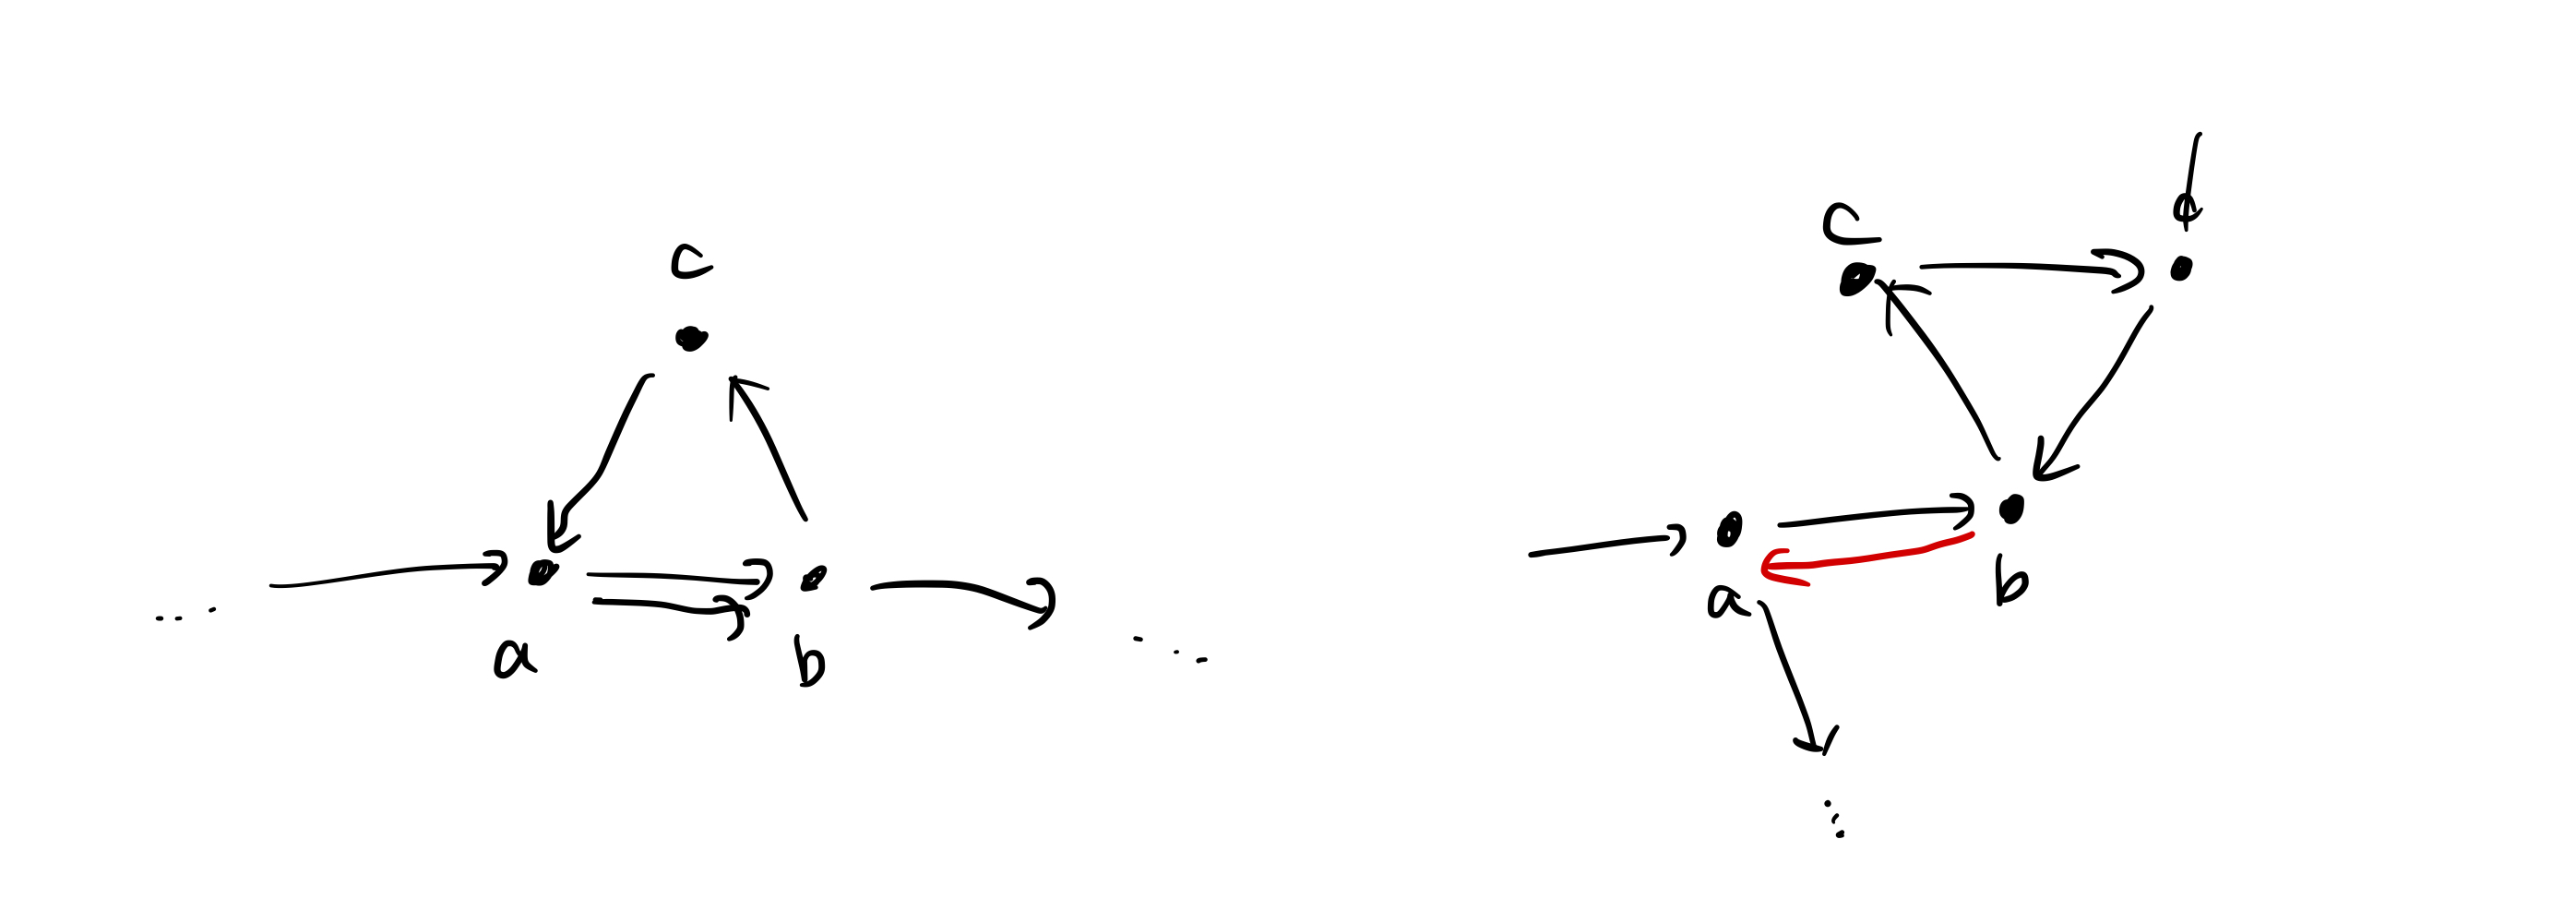
\includegraphics[width=0.66\textwidth]{backtrack.png}
    \caption{右の路は辺$\{a,b\}$を両方の向きで通過しているためバックトラックする.\label{fig:backtrack}}
    \end{center}
  \end{figure}
\end{problem}

\begin{solution}
  \paragraph*{解説.}
  与えられたグラフを$G=(V,E)$とし, 二頂点を$s,t\in V$とする.
  以下の乱択アルゴリズムを考える:
  \begin{enumerate}
    \item 全ての辺$e=\{u,v\}\in E$に一様ランダムに向きを付けて$(u,v)$または$(v,u)$のどちらかを選ぶ. このようにして得られた有向グラフを$G'=(V,E')$とする.
    \item $G'$の有向隣接行列を$B$とする. すなわち, $G'$が辺$(u,v)$含むとき$B_{u,v}=1$であり, それ以外のとき$B_{u,v}=0$とする.
    \item $B^{247}$を計算し, $B^{247}_{s,t}\ge 1$を満たすならば, 「Yes」を出力して終了する.
    \item ステップ1から3を十分大きな定数回, 具体的には $100\cdot 2^{247}$回だけ繰り返し, 一度もYesが出力されなければNoを出力して終了する.
  \end{enumerate}
  このアルゴリズムは確かに$O(n^3)$時間で動作する. また, このアルゴリズムは以下を満たす:
  \begin{itemize}
    \item 入力$G$の答えがYesならば, このアルゴリズムは確率$0.99$でYesを出力する.
    \item 入力$G$の答えがNoならば, このアルゴリズムは確率$1$でNoを出力する.
  \end{itemize}
  これら二つの主張を証明すれば, 上記のアルゴリズムが正しく問題を解くことが示されたことになる.
  
  一つ目の主張を証明する. グラフ$G$がバックトラックしない長さがちょうど$247$の$st$路 $P=(v_0,\dots,v_{247})$ を含むとする. このとき, 確率$2^{-247}$で, ステップ1で得られる有向$G'$においてこの路を構成する全ての辺は$v_i \to v_{i+1}$の向きになる. すなわち, 少なくとも確率$2^{-247}$で$B^{247}_{v_i,v_{i+1}}=1$となるため, アルゴリズムはYesを出力する.

  二つ目の主張を証明する. このとき, 長さ247の任意の$st$路$P=(v_0,\dots,v_{247})$に対し, ある辺$\{u,v\}\in E$が存在して, $P$はこの辺を$u\to v$と$v \to u$の両方の向きで通過する. 従って, どのように向きをつけても$P$は有向グラフ上の路になりえない. すなわち, 確率$1$で$B^{247}_{v_i,v_{i+1}}=0$となるため, アルゴリズムはNoを出力する.

  \paragraph*{すごくズルい別解.} 成功確率が$1/2$以上あればよいので, 入力を見ないで単にYes/Noをランダムに出力すればよい. これは$O(1)$時間でできる (問題文の穴をついたが, 今回の期末課題ではこれでもOKとする).
\end{solution}

\newpage

\begin{problem}
  第6回課題の問1で考えた主問題(P)とその双対問題(D)を考える:
  \begin{center}
    \begin{minipage}{0.4\textwidth}
      \begin{empheq}[box=\fbox]{align*}
            \text{(P)} \quad \text{minimize} \quad & c^\top x \\
        \text{s.t.} \quad & Ax \ge b \\
                          & x \ge 0
      \end{empheq}
    \end{minipage}
    \quad
    \begin{minipage}{0.4\textwidth}
      \begin{empheq}[box=\fbox]{align*}
              \text{(D)} \quad \text{maximize} \quad & y^\top b \\
          \text{s.t.} \quad & y^\top A \le c^\top \\
                            & y \ge 0
        \end{empheq}
    \end{minipage}
  \end{center}

  第6回課題では非負制約$x\ge 0$を関数$\mathcal{L}^*(y):=\inf_{x\ge 0}\{c^\top x + y^\top (b-Ax)\}$に組み込んで(D)を導出した. 今回は非負制約を行列を用いて書き換えた問題(P')について, 第6回講義資料と同様の方法で双対問題を導出せよ:
    \begin{empheq}[box=\fbox]{align*}
        \text{(P')} \quad \text{minimize} \quad & c^\top x \\
    \text{s.t.} \quad & \begin{bmatrix} A \\
    I \end{bmatrix} x \ge \begin{bmatrix} b \\
    0 \end{bmatrix}
  \end{empheq}
  ただし, $I\in\mathbb{R}^{n\times n}$は単位行列である. また, $Ax\ge b$に対応する双対変数を$y\in\mathbb{R}^m$, $Ix\ge 0$に対応する双対変数を$z\in\mathbb{R}^n$とせよ.
  さらに, この導出した双対問題を(D')としたとき, (D)と(D')が等価であることを示せ. つまり, 一方の最適解を用いて他方の最適解を構成できることを示せ. (\textbf{10点})

\end{problem}

\begin{solution}
  \paragraph*{解説.}
  (P')の双対問題は以下のように導出できる:
  まず, 行列$A'\in\mathbb{R}^{(m+n)\times n}$を$A'\coloneqq \begin{bmatrix} A \\ I \end{bmatrix}$と定義する. 
  同様に, ベクトル$b'\in\mathbb{R}^{m+n}$を$b'\coloneqq \begin{bmatrix} b \\ 0 \end{bmatrix}$と定義する.
  $Ax\ge b$に対応する双対変数を$y\in\mathbb{R}^m$, $Ix\ge 0$に対応する双対変数を$z\in\mathbb{R}^n$とする (ただし, $y,z\ge 0$).

  関数
  \begin{align}
    \mathcal{L}^*(y,z):=\inf_{x}\{c^\top x + y^\top (b-Ax) - z^\top x\} \label{eq2}
  \end{align}
  を考える. この関数を式変形すると
  \begin{align}
    \mathcal{L}^*(y,z) &= y^\top b + \inf_{x}\{(c^\top - y^\top A - z^\top)x\} \nonumber\\
                      &= \begin{cases}
                        y^\top b & \text{if } c^\top - y^\top A - z^\top = 0 \\
                        -\infty & \text{otherwise}
                      \end{cases} \label{eq3}
  \end{align}
  となる. 従って双対問題(D')は以下のようになる:
  \begin{empheq}[box=\fbox]{align*}
    \text{(D')} \quad \text{maximize} \quad & y^\top b \\
    \text{s.t.} \quad & y^\top A + z^\top = c^\top \\
                      & y \ge 0 \\
                      & z \ge 0
  \end{empheq}

  次に(D)と(D')が等価であることを示す. (D)の最適解を$y^*\in\mathbb{R}^m$とする. このとき, $(z^*)^\top=c^\top - y^\top A$とすれば, $(y^*,z^*)$は(D')の最適解となる. 実際, $(y^*,z^*)$は確かに(D')の実行可能解であり, これがもし(D')の最適解でないとすると、(D')の別の実行可能解$(y',z')$が存在して$(y')^\top b > (y^*)^\top b$となる. しかしながら, $y'$は(D)の実行可能解でもあり, (D')と同じ目的関数値を持つため, $y^*$が(D)の最適解であることに矛盾する.
  
  一方で, (D')の最適解$(y^*,z^*)$に対し, $y^*$は(D)の最適解となる. 最適性は上と同様.
\end{solution}
\end{document}
